\documentclass[shownotes notes,intlimits]{beamer}


\mode<presentation>
{
  \usetheme[footline]{UAFshade}
  \setbeamercovered{transparent}
}

% load packages
\usepackage{multimedia}
\usepackage{animate}
\usepackage[english]{babel}
\usepackage[latin1]{inputenc}
\usepackage[T1]{fontenc}
\usepackage{lmodern}
\usepackage[multidot]{grffile}

\usepackage{tikz}
\usetikzlibrary{shapes,arrows,shadows, calc}

\usepackage{pgfpages}
\setbeamertemplate{note page}[plain]
\setbeameroption{show notes on second screen=right}


\definecolor{dark red}{HTML}{E41A1C}
\definecolor{dark green}{HTML}{4DAF4A}
\definecolor{dark violet}{HTML}{984EA3}
\definecolor{dark blue}{HTML}{084594}
\definecolor{dark orange}{HTML}{FF7F00}
\definecolor{light blue}{HTML}{377EB8}
\definecolor{light red}{HTML}{FB9A99}
\definecolor{light violet}{HTML}{CAB2D6}

\definecolor{uaf red}{HTML}{E41A1C}
\definecolor{uaf blue}{HTML}{377EB8}
\definecolor{uaf green}{HTML}{4DAF4A}
\definecolor{uaf violet}{HTML}{984EA3}
\definecolor{uaf orange}{HTML}{FF7F00}
\setbeamercolor{boxed}{fg=black,bg=uaf yellow}

\graphicspath{{figures/}}

\setbeamerfont{caption}{size=\scriptsize}

% code adapted from http://tex.stackexchange.com/a/11483/3954

% some parameters for customization
\def\shadowshift{3pt,-3pt}
\def\shadowradius{6pt}

\colorlet{innercolor}{black!60}
\colorlet{outercolor}{gray!05}

% this draws a shadow under a rectangle node
\newcommand\drawshadow[1]{
    \begin{pgfonlayer}{shadow}
        \shade[outercolor,inner color=innercolor,outer color=outercolor] ($(#1.south west)+(\shadowshift)+(\shadowradius/2,\shadowradius/2)$) circle (\shadowradius);
        \shade[outercolor,inner color=innercolor,outer color=outercolor] ($(#1.north west)+(\shadowshift)+(\shadowradius/2,-\shadowradius/2)$) circle (\shadowradius);
        \shade[outercolor,inner color=innercolor,outer color=outercolor] ($(#1.south east)+(\shadowshift)+(-\shadowradius/2,\shadowradius/2)$) circle (\shadowradius);
        \shade[outercolor,inner color=innercolor,outer color=outercolor] ($(#1.north east)+(\shadowshift)+(-\shadowradius/2,-\shadowradius/2)$) circle (\shadowradius);
        \shade[top color=innercolor,bottom color=outercolor] ($(#1.south west)+(\shadowshift)+(\shadowradius/2,-\shadowradius/2)$) rectangle ($(#1.south east)+(\shadowshift)+(-\shadowradius/2,\shadowradius/2)$);
        \shade[left color=innercolor,right color=outercolor] ($(#1.south east)+(\shadowshift)+(-\shadowradius/2,\shadowradius/2)$) rectangle ($(#1.north east)+(\shadowshift)+(\shadowradius/2,-\shadowradius/2)$);
        \shade[bottom color=innercolor,top color=outercolor] ($(#1.north west)+(\shadowshift)+(\shadowradius/2,-\shadowradius/2)$) rectangle ($(#1.north east)+(\shadowshift)+(-\shadowradius/2,\shadowradius/2)$);
        \shade[outercolor,right color=innercolor,left color=outercolor] ($(#1.south west)+(\shadowshift)+(-\shadowradius/2,\shadowradius/2)$) rectangle ($(#1.north west)+(\shadowshift)+(\shadowradius/2,-\shadowradius/2)$);
        \filldraw ($(#1.south west)+(\shadowshift)+(\shadowradius/2,\shadowradius/2)$) rectangle ($(#1.north east)+(\shadowshift)-(\shadowradius/2,\shadowradius/2)$);
    \end{pgfonlayer}
}

% create a shadow layer, so that we don't need to worry about overdrawing other things
\pgfdeclarelayer{shadow} 
\pgfsetlayers{shadow,main}

\newsavebox\mybox
\newlength\mylen

\newcommand\shadowimage[2][]{%
\setbox0=\hbox{\includegraphics[#1]{#2}}
\setlength\mylen{\wd0}
\ifnum\mylen<\ht0
\setlength\mylen{\ht0}
\fi
\divide \mylen by 120
\def\shadowshift{\mylen,-\mylen}
\def\shadowradius{\the\dimexpr\mylen+\mylen+\mylen\relax}
\begin{tikzpicture}
\node[anchor=south west,inner sep=0] (image) at (0,0) {\includegraphics[#1]{#2}};
\drawshadow{image}
\end{tikzpicture}}

\newcommand\shadowimagec[3][]{%
\setbox0=\hbox{\includegraphics<#1>[#2]{#3}}
\setlength\mylen{\wd0}
\ifnum\mylen<\ht0
\setlength\mylen{\ht0}
\fi
\divide \mylen by 120
\def\shadowshift{\mylen,-\mylen}
\def\shadowradius{\the\dimexpr\mylen+\mylen+\mylen\relax}
\begin{tikzpicture}
\node[anchor=south west,inner sep=0] (image) at (0,0) {\includegraphics<#1>[#2]{#3}};
\drawshadow{image}
\end{tikzpicture}}


\newenvironment{transbox}[1][]{%
\begin{tikzpicture}
\node[drop shadow,rounded corners,text width=\textwidth,fill=white, fill opacity=#1,text opacity=1] \bgroup
}{
\egroup;\end{tikzpicture}} 

\newenvironment{transbox-tight}{%
\begin{tikzpicture}
\node[drop shadow,rounded corners,fill=uaf yellow, fill opacity=0.75,text opacity=1] \bgroup
}{
\egroup;\end{tikzpicture}} 

% Define block styles
\tikzstyle{decision} = [ellipse, draw, 
    text badly centered, node distance=3cm, inner sep=2pt,draw=dark violet,
        % The filling: 
        top color=white, 
        bottom color=light violet]
\tikzstyle{warm} = [rectangle, draw,
    text badly centered, rounded corners,draw=dark orange,
        % The filling: 
        top color=white, 
        bottom color=dark orange]
\tikzstyle{glacial} = [rectangle, draw,
    text badly centered, rounded corners,draw=dark blue,
        % The filling: 
        top color=white, 
        bottom color=light blue]
\tikzstyle{arrow line} = [draw, -latex']
\tikzstyle{line} = [draw]


% title page
\title[] % (optional, use only with long paper titles)
{Chronicles of the Greenland Ice Sheet}
\subtitle{An Outlet Glacier Perspective}


\author[Aschwanden] % (optional, use only with lots of authors)
{A.~Aschwanden, M.~Fahnestock, \& C.~Khroulev}
% - Give the names in the same order as the appear in the paper.
% - Use the \inst{?} command only if the authors have different
%   affiliation.

\institute[Geophysical Institute] % (optional, but mostly needed)
{Geophysical Institute, University of Alaska Fairbanks}
% - Use the \inst command only if there are several affiliations.
% - Keep it simple, no one is interested in your street address.

\date{}
\titlegraphic{\vskip-0.5cm\shadowimage[width=\textwidth]{gris-nw-speed-exp-600m}}


\begin{document}

% define what is shown at the beginning of each section
\AtBeginSection[]
{
  \begin{frame}<handout:0>
    \frametitle{Outline}
   \tableofcontents[currentsection,subsectionstyle=hide/hide/hide]
  \end{frame}
}

% define what is shown at the beginning of each subsection
\AtBeginSubsection[]
{
 \begin{frame}<beamer>
  \frametitle{Outline}
   \tableofcontents[currentsection,currentsubsection]
 \end{frame}
}



\setbeamertemplate{background canvas}
  {
     \tikz{\node[inner sep=0pt,opacity=1.0] {\includegraphics[width=\paperwidth]{uaf_beamer_shade_bg}};}
} 


% insert titlepage
\begin{frame}
  \titlepage
  \note[item]{Since the publication of IPCC's Fifth Assessment Report}
  \note[item]{the West Antarctic Ice Sheet has been dominating the news}
  \note[item]{today, I'd like to talk about the long term stability}
  \note[item]{of the Greenland Ice Sheet}
  \note[item]{in terms of SLR potential, I know, it's Antarctica first}
  \note[item]{but \ldots}
\end{frame}

\setbeamertemplate{background canvas}
{
%
} 

\begin{frame}{Recent mass loss from Greenland}
  \begin{columns}
    \column[T]{6cm}
    \begin{itemize}
      \item<1-> about 60\,\% of present-day mass loss occurs through 200+ outlet glaciers (Enderlin et al., 2014)
      \item<2-> yet IPCC AR5 models have not been able to capture outlet glacier flow
      \item<3-> due to poor knowledge of subglacial topography
      \item<4-> radar data collection efforts by NASA's mission Operation Ice Bridge and CReSIS have led to a more detailed picture of the subglacial topography (and ice thickness)
    \end{itemize}
    \column[T]{6cm}
    \vspace{-2.em}
    \begin{figure}
      \includegraphics<1>[height=.85\textheight]{greenland-obs-overview} \only<1>{\\ \scriptsize{Rignot \& Mouginot (2012)}}
      \includegraphics<2>[height=.85\textheight]{greenland-exp-overview-oldbed} \only<2>{\\ \scriptsize{model simulation}}
      \includegraphics<3>[height=.85\textheight]{greenland-obs-basal-overview} \only<3>{\\ \scriptsize{Bamber et al. (2001)}}
      \includegraphics<4>[height=.85\textheight]{greenland-obs-basal-overview-mo14} \only<4>{\\ \scriptsize{Morlighem et al. (2014)}}
    \end{figure}
  \end{columns}
  \note<1>[item]{Here we have observed surface speeds on a log scale,}
  \note<1>[item]{where purple and red colors indicate fast flow}
  \note<2>[item]{now, if we look at a model simulation representative of that time}
  \note<2>[item]{we see that the bigger picture isn't that bad but when we zoom in}
  \note<2>[item]{it becomes evident that we are not able to capture the fast flow in outlet glaciers}
  \note<3>[item]{the reason for such a poor model performance was poor knowledge of subglacial topography}
  \note<3>[item]{we know from Glaciology 100 that ice thickness is the major constraint on ice flow}
  \note<3>[item]{so no surprise there}
  \note<3>[item]{again focusing on Jakobshavn, we see that no channel is evident}
  \note<3>[item]{In 2008, NASA started a large ice thickness data collection campaign}
  \note<3>[item]{as part of their Mission Operation Ice Bridge, together with CReSIS}
  \note<4>[item]{since then, thousands of km of radar profiles have been collected}
  \note<4>[item]{which has resulted in a much more detailed picture of the subglacial topography}
\end{frame}

\begin{frame}{Beneath most outlet glaciers, there is a through}
\vspace{-1.5em}
  \begin{columns}
    \column[T]{5cm}
    \begin{figure}
      \includegraphics<1>[height=.75\textheight]{greenland-obs-overview} \\
      {\scriptsize 
      Observed speeds (Rignot \& Mouginot, 2012)}
    \end{figure}
    \column[T]{5cm}
    \begin{figure}
      \includegraphics<1>[height=.75\textheight]{greenland-obs-basal-overview-mo14} \\
      {\scriptsize
      Subglacial topography (Morlighem et al., 2014)}
    \end{figure}
  \end{columns}
  \note[item]{today we know that outlet glaciers flow in deep channels}
\end{frame}


\begin{frame}{Capturing outlet glacier flow}
\vspace{-.5em}
    \begin{figure}
      \includegraphics<1>[width=0.95\textwidth]{greenland-overview-3} \\
      {\scriptsize Aschwanden, Fahnestock \& Truffer (2016, Nature Comms.)}
    \end{figure}
    \note[item]{Now with the availability of high-resolution ice thickness measurements}
    \note[item]{we wanted to know how much better ice sheet models}
    \note[item]{have become at capturing outlet glacier flow}
    \note[item]{so we combined an open-source ice sheet model capable}
    \note[item]{of outlet-glacier resolving resolution}
    \note[item]{with a high-res ice thickness map}
    \note[item]{We compare observed and modeled flow across selected outlet glaciers}
    \note[item]{We found that outlet glacier flow is well captured by the model if}
    \note[item]{both where ice thickness is well constrained AND}
    \note[item]{model resolution is high enough}
\end{frame}



\begin{frame}{Where are the projections?}

\begin{block}{Now that we have outlet glaciers, we could do new projections}
  \begin{itemize}
  \item technically easy to to, but issues with model initialization
  \end{itemize}
\end{block}

\begin{block}{1-century-scale}
  \begin{itemize}
  \item technically easy to to, but issues with model initialization
  \end{itemize}
\end{block}


\begin{block}{multi-century to millennia-scale}
  \begin{itemize}
  \item technically easy to to, but issues with model initialization
  \end{itemize}
\end{block}
\end{frame}

\begin{frame}{Role of outlet glaciers}

\end{frame}

\begin{frame}{Model Calibration}
  \begin{block}{Atmosphere, Isostasy}
    \begin{itemize}
    \item calibrated at 9,000\,m resolution
    \end{itemize}
  \end{block}
  \begin{block}{Ocean}
    \begin{itemize}
    \item calibrated at 6,000\,m resolution
    \item calving (\alert{stress}-, eigen-calving)
    \item \alert{multi-year sea ice parametrized via back-pressure}
    \item \alert{sub-shelf and frontal melt} parametrization tied to atmosphere temperature
    \end{itemize}
  \end{block}
    \alert{*new model physics}
    \note[item]{We're standing here on the shoulder of giants}
    \note[item]{who have paved the way}
\end{frame}


\begin{frame}{LGM}
  \begin{columns}
    \column[T]{5cm}
    \vspace{-2em}
    \begin{figure}
      \only<1>{\scriptsize{18,000m, SIA}\\}
      \only<2>{\scriptsize{18,000m}\\}
      \only<3>{\scriptsize{9,000m}\\}
      \only<4>{\scriptsize{6,000m}\\}
      \only<5>{\scriptsize{4,500m}\\}
      \only<6>{\scriptsize{3,600m}\\}
      \only<7>{\scriptsize{3,000m}\\}
      \only<8>{\scriptsize{2,400m}\\}
      \only<9>{\scriptsize{1,800m}\\}
      \includegraphics<1>[height=0.8\textheight]{lgm_cc_speed_18000m_sia_ws}
      \includegraphics<2>[height=0.8\textheight]{lgm_cc_speed_18000m_ws}
      \includegraphics<3>[height=0.8\textheight]{lgm_cc_speed_9000m_ws}
      \includegraphics<4>[height=0.8\textheight]{lgm_cc_speed_6000m_ws}
      \includegraphics<5>[height=0.8\textheight]{lgm_cc_speed_4500m_ws}
      \includegraphics<6>[height=0.8\textheight]{lgm_cc_speed_3600m_ws}
      \includegraphics<7>[height=0.8\textheight]{lgm_cc_speed_3000m_ws}
      \includegraphics<8>[height=0.8\textheight]{lgm_cc_speed_2400m_ws}
      \includegraphics<9>[height=0.8\textheight]{lgm_cc_speed_1800m_ws}
    \end{figure}
    \column[T]{5cm}
    \vspace{-2em}
    \begin{figure}
      \only<9>{\scriptsize{18,000m, SIA}\\}
      \includegraphics<9>[height=0.8\textheight]{lgm_cc_speed_18000m_sia_ws}
    \end{figure}
  \end{columns}
\end{frame}

% \begin{frame}{Simulated ice discharge by basin}
%   \begin{columns}
%     \column[T]{4cm}
%     \begin{itemize}
%       \item $2-4$ fold increase
%     \end{itemize}
%     \column[T]{6cm}
%     \vspace{-1em}
%     \begin{figure}
%       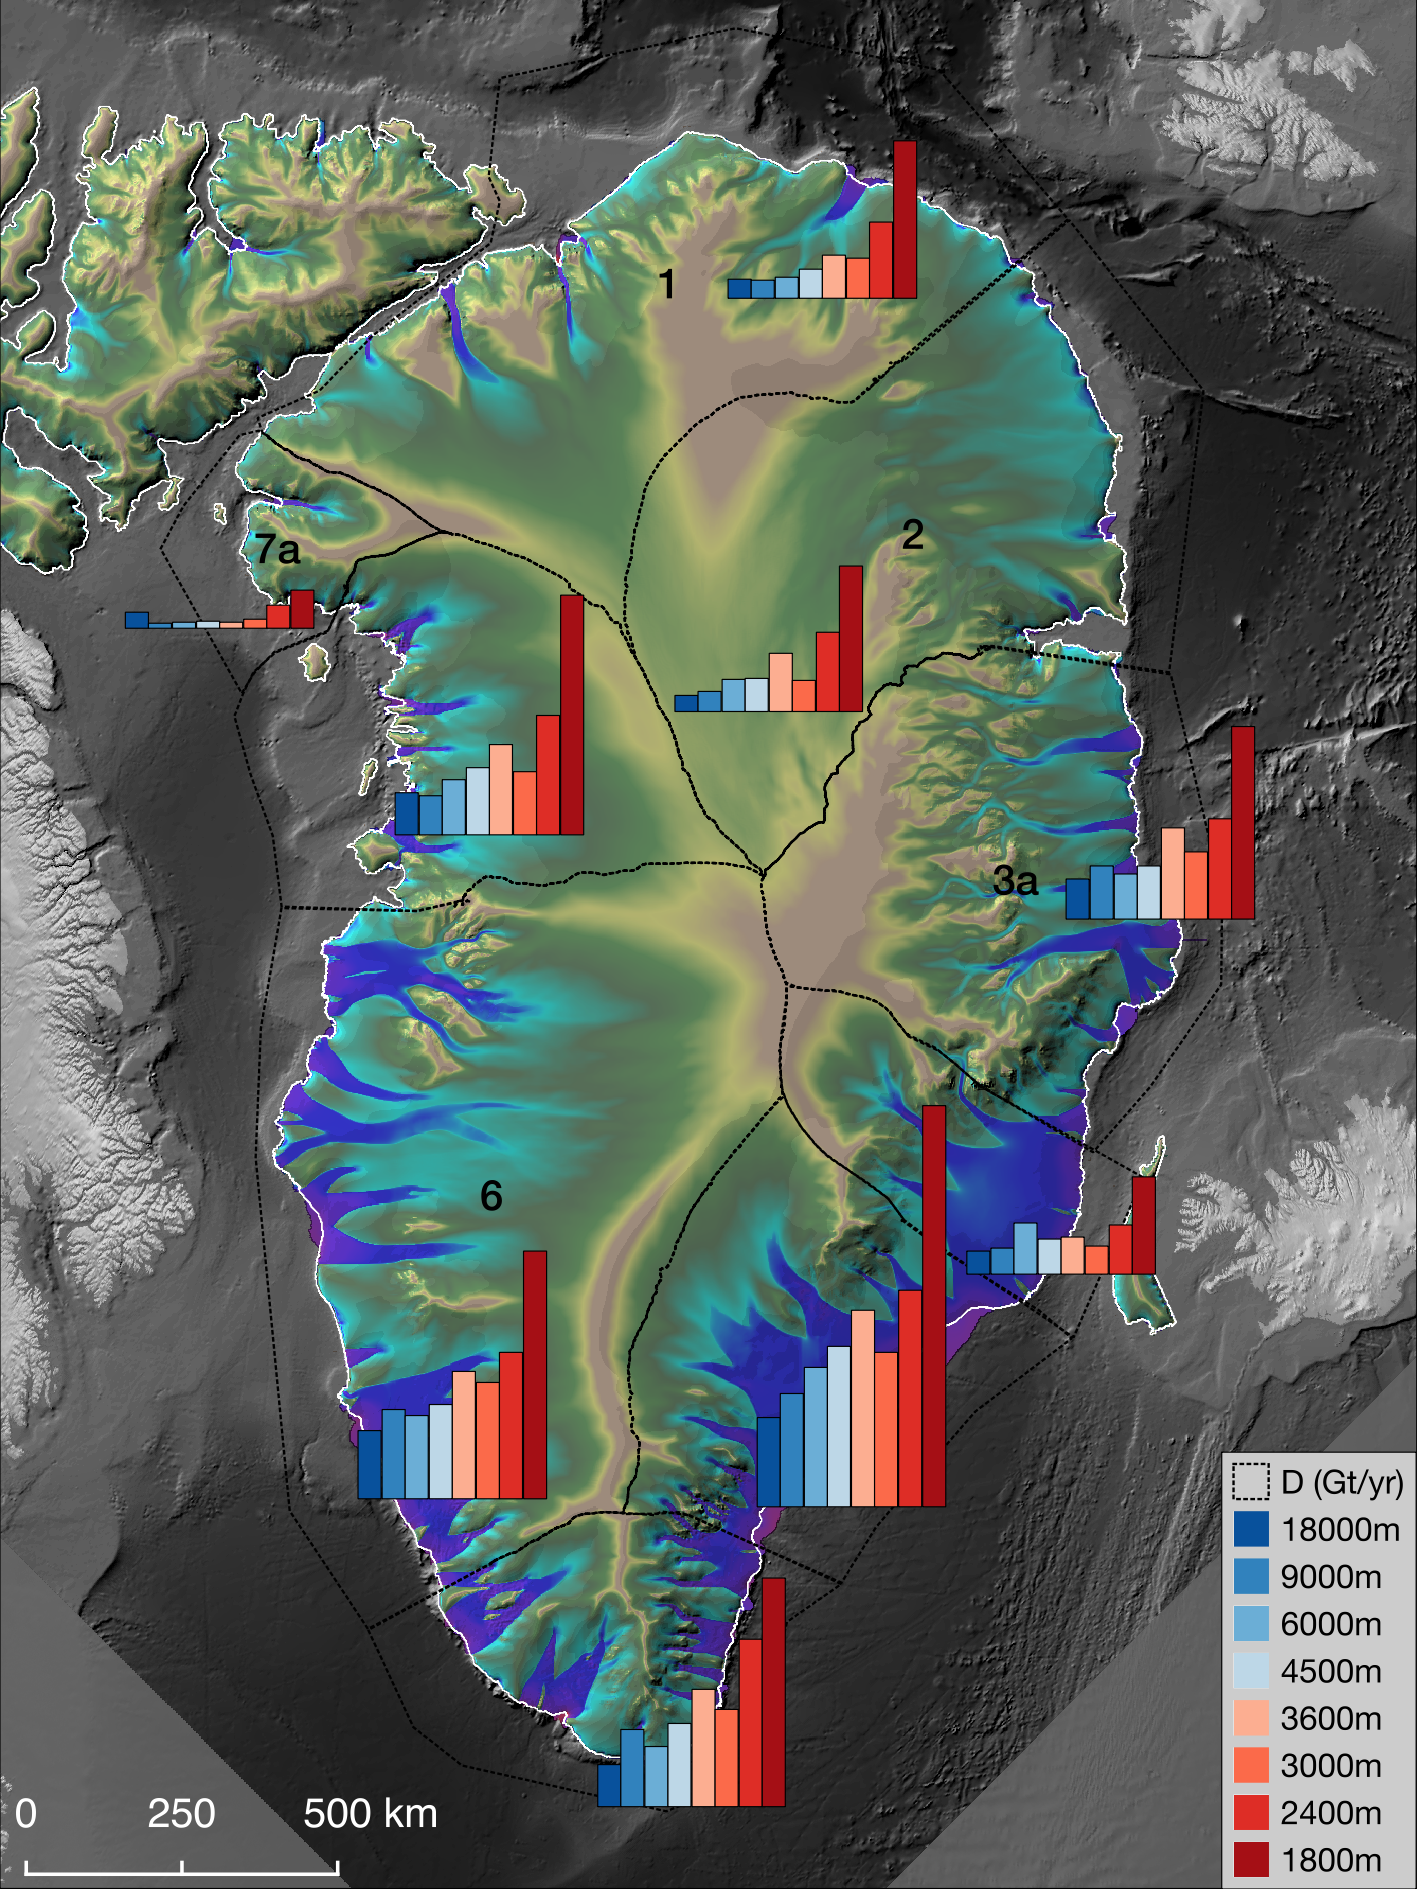
\includegraphics[height=0.85\textheight]{lgm_cc_d_hist}
%     \end{figure}
%   \end{columns}
% \end{frame}

\begin{frame}{Abrupt glacial/inter-glacial}
  \vspace{1em}
  
\begin{tikzpicture}[node distance = 2cm, auto]
    % Place nodes
    \node  (start) {};
    \node [warm, right of =start, node distance=2.5cm] (present day) {present-day};
    \node [glacial, right of=present day, node distance=4cm] (glacial) {glacial};
    \node [warm, right of=glacial, node distance=4cm] (warm) {warm};
    % edges
    \path [line] (present day) -- (glacial);
    \path [line] (glacial) -- (warm);
  \end{tikzpicture}
  \begin{figure}
    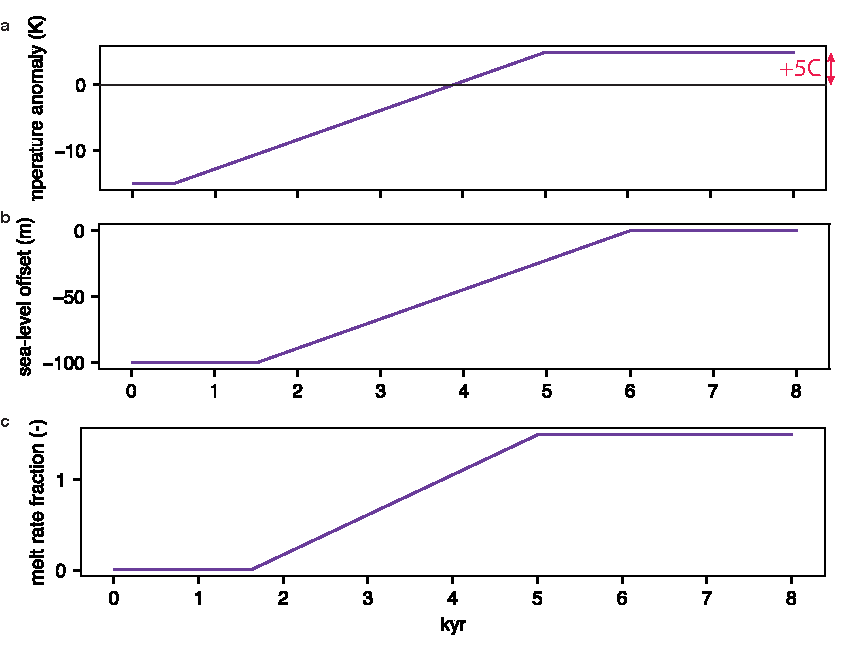
\includegraphics[width=9cm]{glacial_forcing_ts}
  \end{figure}
\end{frame}

\begin{frame}{Acknowledgments}
  \begin{block}{Inspiration}
    \begin{itemize}
      \item Martin Truffer (UAF)
      \item Abbas Khan (DTU Space)
      \item Kurt Kj{\ae}r, Kristian Kjeldsen (Nat. History Museum, Copenhagen)
    \end{itemize}
  \end{block}
  \begin{block}{Funding}
    \begin{figure}
      
\includegraphics[width=2cm]{nasa-logo}
    \end{figure}
  \end{block}
\end{frame}

\end{document}
